\documentclass{ximera}

\title{Increasing and Decreasing Functions Activity}
\author{MATH 425: Calculus I}

\begin{document}
\begin{abstract}
   Working with the peers in your group, solve the following problems. Make sure to show and justify all your work. Make sure everyone in the group understands the solution and participates. Be prepared to report your answers to the whole class. 
\end{abstract}
\maketitle


\begin{exercise}
    Find all intervals of increasing and decreasing for the function $f(x)=3x^5-5x^3$.  Identify any local extrema.
\end{exercise}

\begin{exercise}
    Let $h(x)=\frac{1}{3}x^3-5x^2+24x+2$. Find the intervals of increase and decrease for $h$ and identify any local extrema.
\end{exercise}

\begin{exercise}
     Suppose that $g$ is a function whose first derivative is \[g'(x)=\frac{(x+4)(x-2)}{x^2+1}.\]
    \begin{enumerate}
        \item Determine, with justification, all critical numbers of $g$.
        \item  By developing a carefully labeled first derivative sign chart, decide whether $g$ has as a local maximum, local minimum, or neither at each critical number.
        \item Does $g$ have a global maximum? global minimum? Justify your claims.
        \item Sketch a possible graph of $y=g(x)$. Clearly label any local or global extrema on the graph.\\
    Problem from Boelkins, et al., \textit{Active Calculus}, 2nd ed.
    \end{enumerate}
\end{exercise}

\begin{exercise}
    Suppose that $h$ is a differentiable function whose first derivative is given by the graph below.
    \begin{image}
        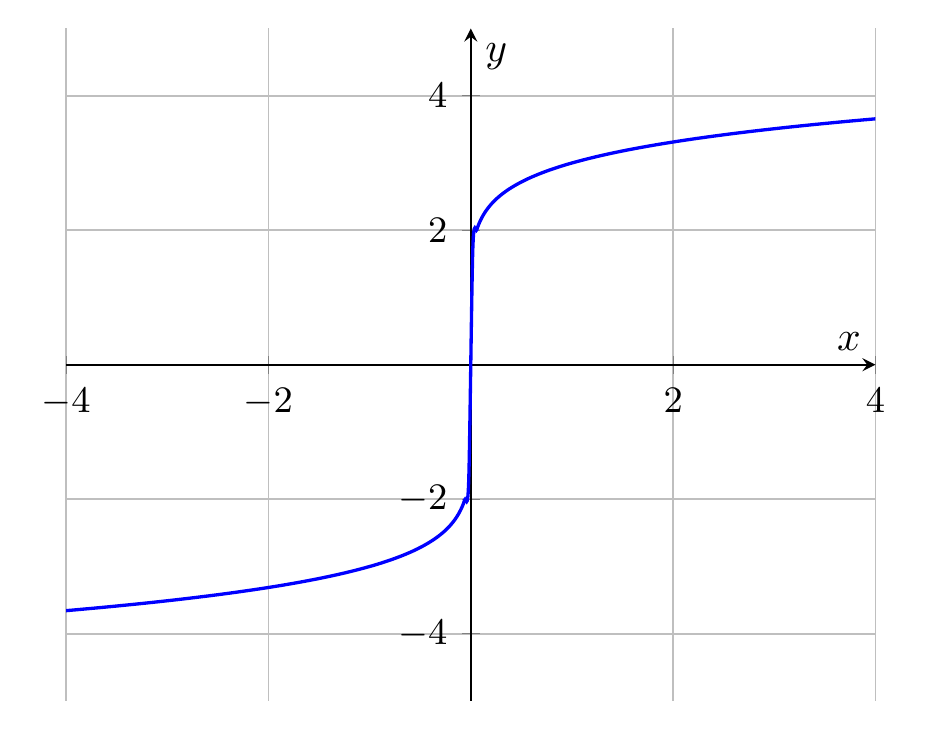
\begin{tikzpicture}[scale=1.5]
            \begin{axis}[
                axis lines=middle,
                xlabel=$x$,
                ylabel=$y$,
                xmin=-4, xmax=4,
                ymin=-5, ymax=5,
                grid=major,
                tick label style={font=\small}
            ]
                \addplot[
                    domain=-4:4,
                    samples=200,
                    smooth,
                    thick,
                    blue
                ] {3*sign(x)*abs(x)^(1/7)};
                %\addlegendentry{$y=3x^{1/9}$}
            \end{axis}
        \end{tikzpicture}  
    \end{image}
    %\xmalt{Graph of a function that is negative and increasing before $x=0$, then positive and increasing after $x=0$. }
    \begin{enumerate}
        \item How many real number solutions can $h$ have? Why? 
        \item If $h(x)$ has two distinct real solutions, what can you say about the signs of the solutions?  Why?
        \item Suppose that $\lim_{x\rightarrow \infty}h'(x)=4$, as appears to be indicated by the graph. What can you say about the behavior of $h$ as $x\rightarrow \infty$?  Justify your answer.
    \end{enumerate}
\end{exercise}



\end{document}
